\documentclass[a4paper,12pt]{article}
\usepackage[utf8]{inputenc}
\usepackage{graphicx}
\usepackage{listings}
\usepackage{amsmath}
\usepackage{geometry}
\geometry{margin=1in}
\usepackage{caption}
\usepackage{float}
\usepackage{subcaption}
\usepackage{hyperref}

\title{Desain dan Implementasi FIR High-Pass Filter pada FPGA DE10-Lite}
\author{Rayhan Rizqi Zamzamy \\ 5022231078}
\date{26 Juni 2025}

\begin{document}

\maketitle

\section{Spesifikasi dan Desain Filter}

Desain dilakukan menggunakan Python (\texttt{scipy.signal.firwin}) untuk mendapatkan koefisien, 
kemudian dikuantisasi ke 16-bit signed integer agar kompatibel dengan VHDL.

\begin{itemize}
    \setlength\itemsep{0em}
    \item \textbf{Bandwidth sinyal input:} 10~kHz
    \item \textbf{Frekuensi cut-off:} 1000 + (angka NRP terakhir $\times$ 100) = 1800~Hz
    \item \textbf{Input:} ADC pada board DE10-Lite (12-bit)
    \item \textbf{Output:} 12-bit digital dari filter
    \item \textbf{Metode desain:} Windowing FIR (Hamming)
\end{itemize}

\vspace{-2em}
\begin{figure}[H]
    \centering
    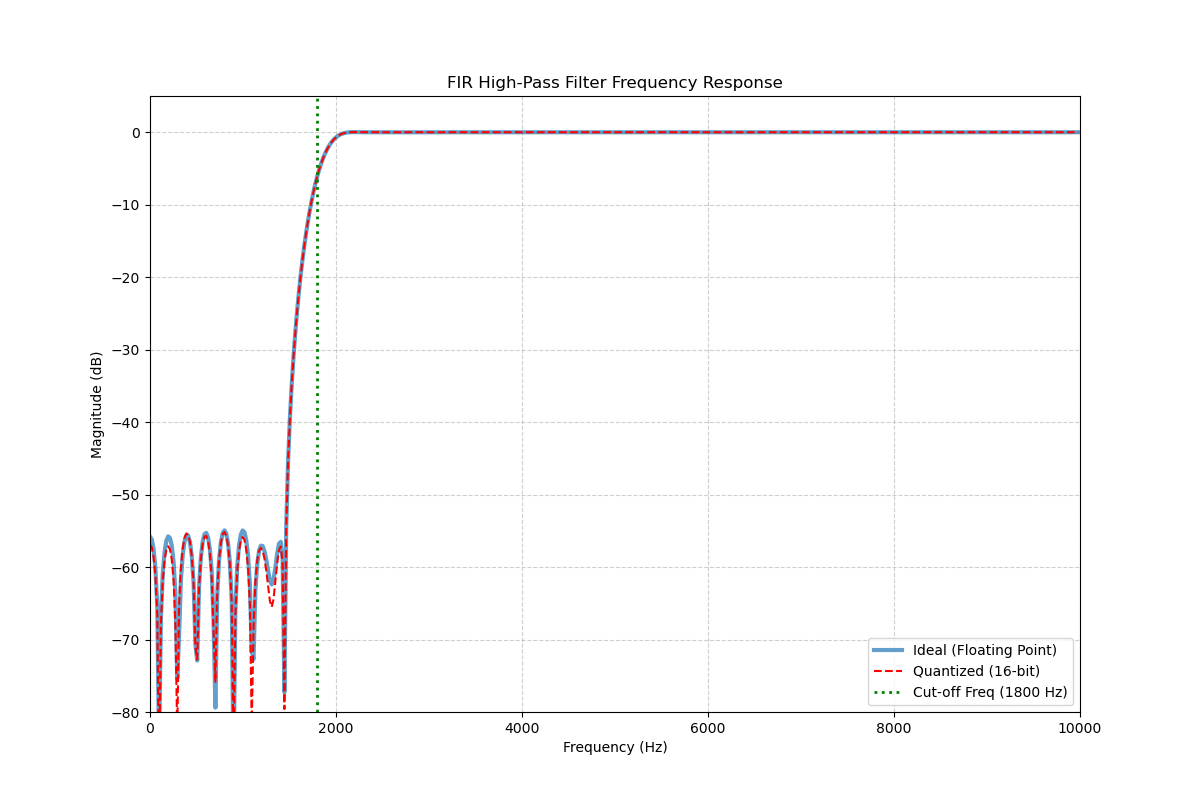
\includegraphics[width=0.5\textwidth]{images/freq_response_sim.png}
    \caption{Respons frekuensi filter FIR high-pass hasil desain Python.}
\end{figure}
\vspace{-2em}

\section{Implementasi pada FPGA}

Implementasi filter FIR dilakukan dalam VHDL dengan arsitektur RTL. 
Modul utama terdiri dari \texttt{fir\_filter}, \texttt{uart\_tx}, \texttt{tx\_packet\_gen}, dan \texttt{de10\_lite\_adc} (IP). 
\texttt{fir\_filter} mengimplementasikan filter FIR dengan koefisien yang telah dikuantisasi. 
\texttt{tx\_packet\_gen} mengemas data menjadi paket yang siap dikirim---terdiri dari 1 byte SoF (\texttt{0xAA}) 
dan 3 byte data tanpa padding: 12-bit input \& 12-bit output.
\texttt{uart\_tx} digunakan untuk mengirim data hasil filter melalui UART dengan baudrate 1 Mbps.
ADC di-sample pada 20 kHz sesuai teori Nyquist (minimum). Dengan baudrate 1 Mbps, data rate maksimum adalah 100 kBps. 
Dengan skema 4 byte per paket, data rate efektif adalah 20 kHz $\times$ 4 byte = 80 kBps---masih ada headroom untuk transmisi yang stabil.

\begin{lstlisting}[language=VHDL, basicstyle=\tiny, lineskip=0em,belowskip=0em,aboveskip=0em, frame=single]
library ieee;
use ieee.std_logic_1164.all;
use ieee.numeric_std.all;

entity fir_filter is
    generic (
        NUM_TAPS              : integer := 101;
        COEFFICIENT_WIDTH     : integer := 16;
        INPUT_WIDTH           : integer := 12;
        OUTPUT_WIDTH          : integer := 12;
        ACCUMULATOR_WIDTH     : integer := 35
    );
    port (
        clk_i           : in  std_logic;
        rst_i           : in  std_logic;
        sample_i        : in  std_logic_vector(INPUT_WIDTH-1 downto 0);
        sample_valid_i  : in  std_logic;
        filtered_o      : out std_logic_vector(OUTPUT_WIDTH-1 downto 0);
        filtered_valid_o: out std_logic
    );
end entity fir_filter;

architecture rtl of fir_filter is
    type T_COEFF_ARRAY is array (0 to NUM_TAPS-1) of signed(COEFFICIENT_WIDTH-1 downto 0);
    constant C_FIR_COEFFS : T_COEFF_ARRAY := (to_signed(0, 16), to_signed(-9, 16), ...);
    type T_DELAY_LINE is array (0 to NUM_TAPS-1) of signed(INPUT_WIDTH-1 downto 0);
    signal s_delay_line : T_DELAY_LINE;
begin
    fir_process: process(clk_i, rst_i)
        variable v_accumulator : signed(ACCUMULATOR_WIDTH-1 downto 0);
    begin
        if (rst_i = '1') then
            s_delay_line <= (others => (others => '0'));
            filtered_valid_o <= '0';
        elsif rising_edge(clk_i) then
            filtered_valid_o <= '0';
            if (sample_valid_i = '1') then
                s_delay_line(1 to NUM_TAPS-1) <= s_delay_line(0 to NUM_TAPS-2);
                s_delay_line(0) <= signed(sample_i);
                v_accumulator := (others => '0');
                for i in 0 to NUM_TAPS-1 loop
                    v_accumulator := v_accumulator + (s_delay_line(i) * C_FIR_COEFFS(i));
                end loop;
                filtered_o <= std_logic_vector(v_accumulator(26 downto 15));
                filtered_valid_o <= '1';
            end if;
        end if;
    end process fir_process;
end architecture rtl;
\end{lstlisting}
\vspace{-1.5em}
\begin{center}
    \captionof{lstlisting}{Kode VHDL untuk modul filter FIR.}
\end{center}
\vspace{-1.5em}

\begin{lstlisting}[language=VHDL, basicstyle=\tiny, lineskip=0em,belowskip=0em,aboveskip=0em, frame=single]
library ieee;
use ieee.std_logic_1164.all;
use ieee.numeric_std.all;

entity uart_tx is
    generic (
        CLK_FREQ     : integer := 50_000_000;
        BAUD_RATE    : integer := 1_000_000
    );
    port (
        clk_i       : in  std_logic;
        rst_i       : in  std_logic;
        tx_start_i  : in  std_logic;
        data_i      : in  std_logic_vector(7 downto 0);
        tx_busy_o   : out std_logic;
        tx_o        : out std_logic
    );
end entity uart_tx;

architecture rtl of uart_tx is
    constant CLK_PER_BIT : integer := CLK_FREQ / BAUD_RATE;
    type T_STATE is (ST_IDLE, ST_START_BIT, ST_DATA_BITS, ST_STOP_BIT);
    signal s_state : T_STATE := ST_IDLE;
    signal s_clk_counter : integer range 0 to CLK_PER_BIT - 1 := 0;
    signal s_bit_counter : integer range 0 to 7 := 0;
    signal s_data_reg    : std_logic_vector(7 downto 0) := (others => '0');
    signal s_tx_busy     : std_logic := '0';
begin
    tx_busy_o <= s_tx_busy;
    uart_process: process(clk_i, rst_i)
    begin
        if (rst_i = '1') then
            s_state       <= ST_IDLE;
            s_clk_counter <= 0;
            s_bit_counter <= 0;
            s_tx_busy     <= '0';
            tx_o          <= '1';
        elsif rising_edge(clk_i) then
            case s_state is
                when ST_IDLE =>
                    s_tx_busy <= '0';
                    tx_o      <= '1';
                    if (tx_start_i = '1') then
                        s_data_reg    <= data_i;
                        s_clk_counter <= 0;
                        s_tx_busy     <= '1';
                        s_state       <= ST_START_BIT;
                    end if;
                when ST_START_BIT =>
                    tx_o <= '0';
                    if (s_clk_counter = CLK_PER_BIT - 1) then
                        s_clk_counter <= 0;
                        s_bit_counter <= 0;
                        s_state       <= ST_DATA_BITS;
                    else
                        s_clk_counter <= s_clk_counter + 1;
                    end if;
                when ST_DATA_BITS =>
                    tx_o <= s_data_reg(s_bit_counter);
                    if (s_clk_counter = CLK_PER_BIT - 1) then
                        s_clk_counter <= 0;
                        if (s_bit_counter = 7) then
                            s_state <= ST_STOP_BIT;
                        else
                            s_bit_counter <= s_bit_counter + 1;
                        end if;
                    else
                        s_clk_counter <= s_clk_counter + 1;
                    end if;
                when ST_STOP_BIT =>
                    tx_o <= '1';
                    if (s_clk_counter = CLK_PER_BIT - 1) then
                        s_clk_counter <= 0;
                        s_state       <= ST_IDLE;
                    else
                        s_clk_counter <= s_clk_counter + 1;
                    end if;
            end case;
        end if;
    end process uart_process;
end architecture rtl;
\end{lstlisting}
\vspace{-1.5em}
\begin{center}
    \captionof{lstlisting}{Kode VHDL untuk modul transmiter UART.}
\end{center}
\vspace{-1.5em}

\begin{lstlisting}[language=VHDL, basicstyle=\tiny, lineskip=0em,belowskip=0em,aboveskip=0em, frame=single]
library ieee;
use ieee.std_logic_1164.all;
use ieee.numeric_std.all;

entity tx_packet_gen is
    port (
        clk_i              : in  std_logic;
        rst_i              : in  std_logic;
        unfiltered_data_i  : in  std_logic_vector(11 downto 0);
        filtered_data_i    : in  std_logic_vector(11 downto 0);
        data_valid_i       : in  std_logic;
        uart_data_o        : out std_logic_vector(7 downto 0);
        uart_start_o       : out std_logic;
        uart_busy_i        : in  std_logic
    );
end entity tx_packet_gen;

architecture rtl of tx_packet_gen is
    type T_STATE is (ST_IDLE, ST_SEND_SYNC, ST_WAIT_SYNC, ST_SEND_BYTE_0, ST_WAIT_BYTE_0,
                     ST_SEND_BYTE_1, ST_WAIT_BYTE_1, ST_SEND_BYTE_2, ST_WAIT_BYTE_2);
    signal s_state      : T_STATE := ST_IDLE;
    signal s_next_state : T_STATE := ST_IDLE;
    constant C_SYNC_BYTE : std_logic_vector(7 downto 0) := x"AA";
    signal r_byte_0 : std_logic_vector(7 downto 0);
    signal r_byte_1 : std_logic_vector(7 downto 0);
    signal r_byte_2 : std_logic_vector(7 downto 0);
begin
    state_reg_proc: process(clk_i, rst_i)
    begin
        if (rst_i = '1') then
            s_state <= ST_IDLE;
        elsif rising_edge(clk_i) then
            s_state <= s_next_state;
            if (data_valid_i = '1') then
                r_byte_0 <= unfiltered_data_i(7 downto 0);
                r_byte_1 <= filtered_data_i(7 downto 0);
                r_byte_2 <= unfiltered_data_i(11 downto 8) & filtered_data_i(11 downto 8);
            end if;
        end if;
    end process state_reg_proc;
    next_state_logic_proc: process(s_state, data_valid_i, uart_busy_i, r_byte_0, r_byte_1, r_byte_2)
    begin
        uart_start_o <= '0';
        uart_data_o  <= (others => '0');
        s_next_state <= s_state;
        case s_state is
            when ST_IDLE =>
                if (data_valid_i = '1' and uart_busy_i = '0') then
                    s_next_state <= ST_SEND_SYNC;
                end if;
            when ST_SEND_SYNC =>
                uart_data_o  <= C_SYNC_BYTE;
                uart_start_o <= '1';
                s_next_state <= ST_WAIT_SYNC;
            when ST_WAIT_SYNC =>
                uart_data_o <= C_SYNC_BYTE;
                if (uart_busy_i = '0') then
                    s_next_state <= ST_SEND_BYTE_0;
                end if;
            when ST_SEND_BYTE_0 =>
                uart_data_o  <= r_byte_0;
                uart_start_o <= '1';
                s_next_state <= ST_WAIT_BYTE_0;
            when ST_WAIT_BYTE_0 =>
                uart_data_o <= r_byte_0;
                if (uart_busy_i = '0') then
                    s_next_state <= ST_SEND_BYTE_1;
                end if;
            when ST_SEND_BYTE_1 =>
                uart_data_o  <= r_byte_1;
                uart_start_o <= '1';
                s_next_state <= ST_WAIT_BYTE_1;
            when ST_WAIT_BYTE_1 =>
                uart_data_o <= r_byte_1;
                if (uart_busy_i = '0') then
                    s_next_state <= ST_SEND_BYTE_2;
                end if;
            when ST_SEND_BYTE_2 =>
                uart_data_o  <= r_byte_2;
                uart_start_o <= '1';
                s_next_state <= ST_WAIT_BYTE_2;
            when ST_WAIT_BYTE_2 =>
                uart_data_o <= r_byte_2;
                if (uart_busy_i = '0') then
                    s_next_state <= ST_IDLE;
                end if;
        end case;
    end process next_state_logic_proc;
end architecture rtl;
\end{lstlisting}
\vspace{-1.5em}
\begin{center}
    \captionof{lstlisting}{Kode VHDL untuk modul generator paket UART.}
\end{center}
\vspace{-1.5em}

\begin{lstlisting}[language=VHDL, basicstyle=\tiny, lineskip=0em,belowskip=0em,aboveskip=0em, frame=single]
library ieee;
use ieee.std_logic_1164.all;
use ieee.numeric_std.all;

entity HighPass_FIR is
    port (
        MAX10_CLK1_50   : in  std_logic;
        KEY             : in  std_logic_vector(1 downto 0);
        ARDUINO_IO      : inout std_logic_vector(15 downto 0);
    );
end entity HighPass_FIR;

architecture rtl of HighPass_FIR is
    constant SAMPLING_RATE_HZ : integer := 20_000;
    constant BAUD_RATE_BPS    : integer := 1_000_000;
    constant CLK_FREQ_HZ      : integer := 50_000_000;
    constant CLK_DIVIDER      : integer := CLK_FREQ_HZ / SAMPLING_RATE_HZ;
    -- Deklarasi komponen. Salin dari file VHDL masing-masing komponen.
    signal clk                : std_logic;
    signal rst                : std_logic;
    signal sample_clk_tick    : std_logic;
    signal adc_ch0_data       : std_logic_vector(11 downto 0);
    signal filtered_data      : std_logic_vector(11 downto 0);
    signal fir_output_valid   : std_logic;
    signal uart_tx_data       : std_logic_vector(7 downto 0);
    signal uart_tx_start      : std_logic;
    signal uart_is_busy       : std_logic;
    signal uart_tx_pin        : std_logic;
begin
    clk <= MAX10_CLK1_50;
    rst <= not KEY(0);
    ARDUINO_IO(1) <= uart_tx_pin;
    sampling_clk_process: process(clk, rst)
        variable v_counter : integer range 0 to CLK_DIVIDER - 1 := 0;
    begin
        if (rst = '1') then
            v_counter       := 0;
            sample_clk_tick <= '0';
        elsif rising_edge(clk) then
            if (v_counter = CLK_DIVIDER - 1) then
                v_counter       := 0;
                sample_clk_tick <= '1';
            else
                v_counter       := v_counter + 1;
                sample_clk_tick <= '0';
            end if;
        end if;
    end process sampling_clk_process;
    adc_inst : component de10_lite_adc
    port map (
        CLOCK => clk,
        RESET => rst,
        CH0   => adc_ch0_data
    );
    fir_inst : component fir_filter
    port map (
        clk_i          => clk,
        rst_i          => rst,
        sample_i       => adc_ch0_data,
        sample_valid_i => sample_clk_tick,
        filtered_o     => filtered_data,
        filtered_valid_o=> fir_output_valid
    );
    packet_inst : component tx_packet_gen
    port map (
        clk_i             => clk,
        rst_i             => rst,
        unfiltered_data_i => adc_ch0_data,
        filtered_data_i   => filtered_data,
        data_valid_i      => fir_output_valid,
        uart_data_o       => uart_tx_data,
        uart_start_o      => uart_tx_start,
        uart_busy_i       => uart_is_busy
    );
    uart_inst : component uart_tx
    generic map (
        CLK_FREQ  => CLK_FREQ_HZ,
        BAUD_RATE => BAUD_RATE_BPS
    )
    port map (
        clk_i      => clk,
        rst_i      => rst,
        tx_start_i => uart_tx_start,
        data_i     => uart_tx_data,
        tx_busy_o  => uart_is_busy,
        tx_o       => uart_tx_pin
    );
end architecture rtl;
\end{lstlisting}
\vspace{-1.5em}
\begin{center}
    \captionof{lstlisting}{Kode VHDL untuk modul top-level.}
\end{center}
\vspace{-1.5em}

\section{Visualisasi pada Komputer}

Data dari FPGA ditransmisikan melalui UART ke komputer, kemudian divisualisasikan menggunakan Python.
Uji coba dilakukan dengan sinyal sinusoidal pada frekuensi 1 kHz dan 2 kHz, dengan amplitudo 2 Vpp dan offset 1 V.
Dapat dilihat bahwa filter berhasil menghilangkan komponen frekuensi 1 kHz, sementara komponen 3 kHz tetap utuh.
Terlihat juga DC offset (komponen 0 Hz) hilang pada output, sesuai dengan desain filter high-pass.
Untuk uji respons frekuensi, digunakan white noise sebagai input. Data dari FPGA dianalisis menggunakan FFT dari komputer
menggunakan Python, menghasilkan respons frekuensi yang sesuai dengan karakteristik high-pass filter dengan frekuensi cut-off 1.8 kHz.
Walaupun hasil tidak sama seperti simulasi Python, namun masih menunjukkan karakteristik high-pass yang diinginkan.

\begin{figure}[H]
    \centering
    \begin{subfigure}[b]{0.3\textwidth}
        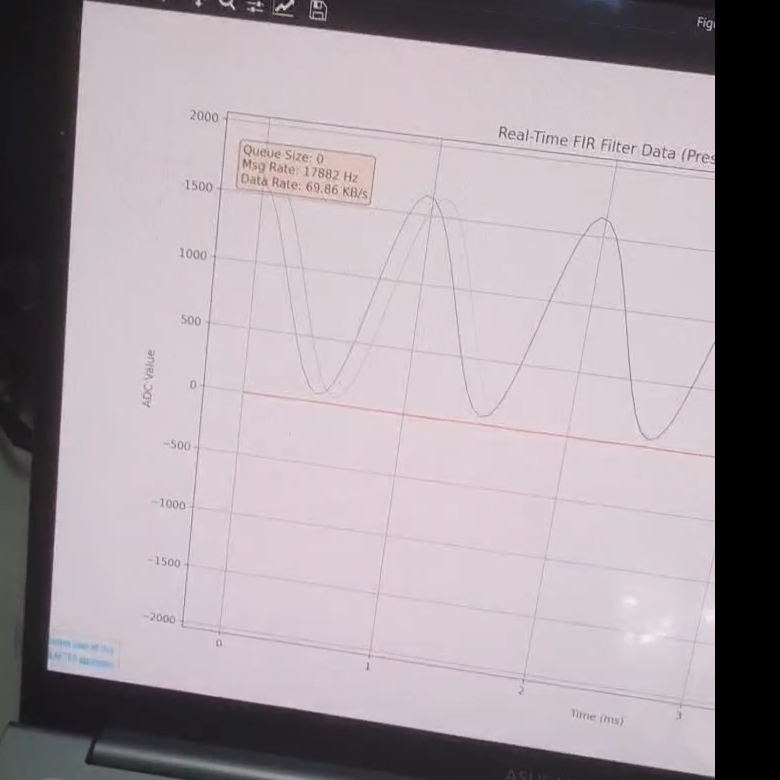
\includegraphics[width=\textwidth]{images/real_stopband_1k.png}
        \caption{Sinusiodal input 1 kHz.}
    \end{subfigure}
    \hfill
    \begin{subfigure}[b]{0.3\textwidth}
        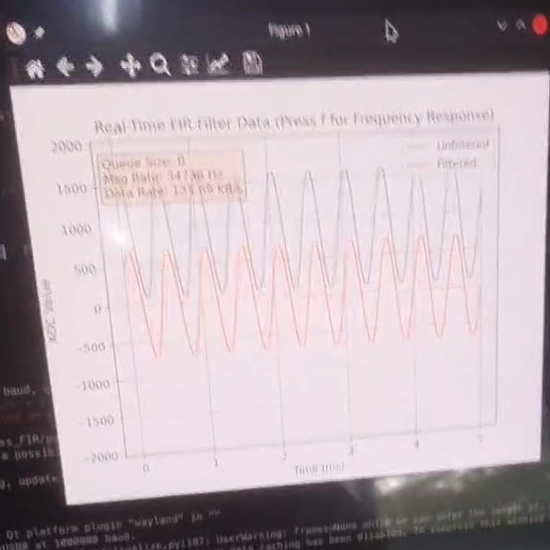
\includegraphics[width=\textwidth]{images/real_passband_2k.png}
        \caption{Sinusiodal input 2 kHz.}
    \end{subfigure}
    \hfill
    \begin{subfigure}[b]{0.3\textwidth}
        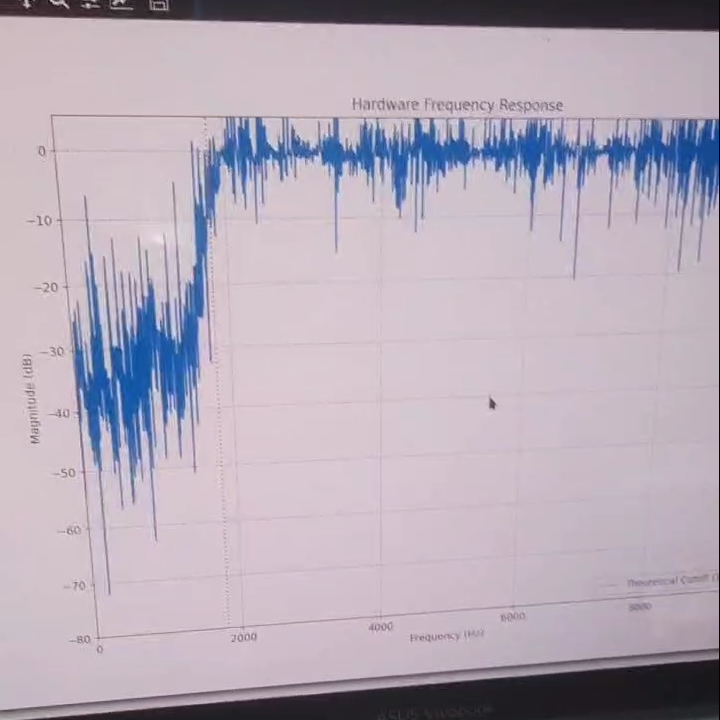
\includegraphics[width=\textwidth]{images/freq_response_real.png}
        \caption{Respons frekuensi filter.}
    \end{subfigure}
    \caption{Visualisasi sinyal input, output, serta respons frekuensi filter.}
\end{figure}

\noindent Catatan: Abaikan metrik data rate, queue, message rate. Kode Python masih bermasalah dalam hal ini,
sehingga tidak valid untuk digunakan sebagai acuan. Fokus pada visualisasi sinyal input dan output,
serta respons frekuensi filter.

\end{document}